\documentclass[a4paper, 12pt]{article}
\usepackage[a4paper,top=1.5cm, bottom=1.5cm, left=1cm, right=1cm]{geometry}
\usepackage{cmap}					% поиск в PDF
\usepackage{mathtext} 				% русские буквы в формулах
\usepackage[T2A]{fontenc}			% кодировка
\usepackage[utf8]{inputenc}			% кодировка исходного текста
\usepackage[english,russian]{babel}	% локализация и переносы

\usepackage{amsmath,amssymb}
\usepackage{indentfirst}
\usepackage{longtable}
\usepackage{graphicx}
\usepackage{array}
\usepackage{float}

\usepackage{floatflt}
\usepackage{wrapfig}
\usepackage{siunitx} % Required for alignment
\usepackage{subfigure}
\usepackage{multirow}
\usepackage{rotating}
\usepackage{caption}

\graphicspath{{.}}


\title{\begin{center}Лабораторная работа №3.2.5\end{center}
Свободные и вынужденные колебания в электрическом контуре}
\author{Рожков А. В.}
\date{\today}

\begin{document}
    \pagenumbering{gobble}
    \maketitle
    \newpage
    \pagenumbering{arabic}
    \renewcommand*{\thesubsection}{\thesection.\Alph{subsection}}

    \textbf{Цель работы:} исследование свободных и вынужденных колебаний в
колебательном контуре.
    \textbf{В работе используются:} осциллограф АКТАКОМ ADS-6142H, генератор сигналов специальной формы АКИП-3409/4, магазин сопротивления МСР-60, магазин емкости Р5025, магазин индуктивности Р567 типа МИСП, соединительная коробка с шунтирующей емкостью, соединительные одножильные и коаксиальные провода.

    \section{Введение}
        \subsection*{Экспериментальная установка}
            Колебательный контур состоит из постоянной индуктивности $L$ с активным сопротивлением $RL$, переменной емкости C и сопротивления $R$. Картина колебаний напряжения на емкости наблюдается на экране двухканального осциллографа. Для возбуждения затухающих колебаний используется генератор сигналов специальной формы. Сигнал с генератора поступает через конденсатор C1 на вход колебательного контура. Данная емкость необходима чтобы выходной импеданс генератора был много меньше импеданса колебательного контура и не влиял на процессы, проходящие в контуре.

            Установка предназначена для исследования не только возбужденных, но и свободных колебаний в электрической цепи. При изучении свободно затухающих колебаний генератор специальных сигналов на вход колебательного контура подает периодические короткие импульсы, которые заряжают конденсатор C. За время между последовательными импульсами происходит разрядка конденсатора через резистор и катушку индуктивности.
            \begin{figure}[H]
                \centering
                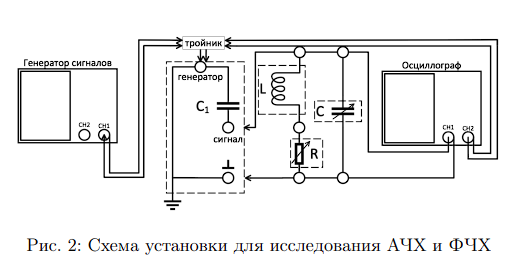
\includegraphics{img/2.png}
            \end{figure}
            \begin{figure}[H]
                \centering
                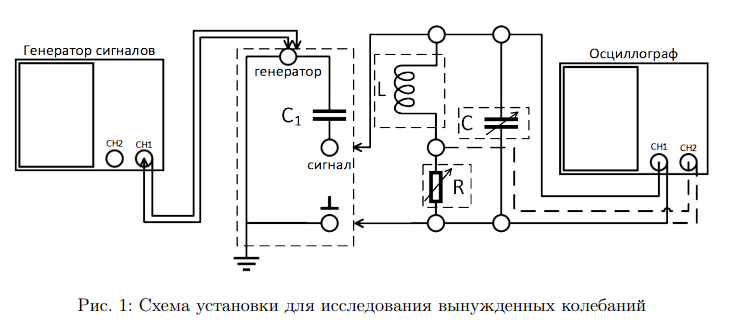
\includegraphics{img/1.png}
            \end{figure}

        \subsection*{Теоретические сведения}

            \noindent Для RLC контура применим правило Кирхгофа:
            \begin{equation}
                RI + U_C + L\frac{dI}{dt} = 0.
            \end{equation}
            Подставив в уравнение выражение для тока через 1-ое правило Кирхгофа разделив обе части уравнения на $CL$, получим:
            \begin{equation}
                \frac{d^2U_C}{dt^2} + \frac{R}{L} \frac{dU_C}{dt} + \frac{U_C}{CL}=0
            \end{equation}
            Произведём замены $\gamma = \frac{R}{2L}$ -- коэффициент затухания, $\omega_0^2 = \frac{1}{LC}$ -- собственная круговая частота, $T_0 = \frac{2\pi}{\omega_0} = 2\pi \sqrt{LC}$ -- период собственных колебаний. Тогда уравнение примет вид:
            \begin{equation}
                \ddot{U_C} + 2 \gamma \dot{U_C} + \omega_0^2U_C = 0,
            \end{equation}
            где точкой обозначено дифференцирование по времени. Будем искать решение данного дифференциального уравнения в классе функций следующего вида:
            $$U_C(t) = U(t)e^{- \gamma t}.$$
            Получим:
            \begin{equation}
                \ddot{U} + \omega_1^2 U = 0,
            \end{equation}
            где
            \begin{equation}
                \omega_1^2 = \omega_0^2-\gamma^2
            \end{equation}
            Для случая $\gamma < \omega_0$ в силу того, что $\omega_1 > 0$, получим:
            \begin{equation}
                U_C(t) = U_0 \cdot e^{-\gamma t} \text{cos}(\omega_1 t + \varphi_0).
            \end{equation}
            Для получения фазовой траектории представим формулу в другом виде:
            \begin{equation}
                U_C(t) = e^{-\gamma t}(a \text{cos} \omega_1 t + b \text{sin} \omega_1 t),
            \end{equation}
            где $a$ и $b$ получаются по формулам:
            $$a = U_0 \text{cos} \varphi_0, \qquad b = - U_0 \text{sin} \varphi_0.$$
            В более удобном виде запишем выражения для напряжения на конденсаторе и токе через катушку:
            \begin{equation}
                U_C (t) = U_{C0} \cdot e^{-\gamma t} (\text{cos} \omega_1 t + \frac{\gamma}{\omega_1} \text{sin} \omega_1 t),
            \end{equation}
            \begin{equation}
                I(t) = C\dot{U_C}= - \frac{U_{C0}}{\rho} \frac{\omega_0}{\omega_1} e^{-\gamma t} \text{sin} \omega_1 t.
            \end{equation}
            Введём некоторые характеристики колебательного движения:
            \begin{equation}
                \tau = \frac{1}{\gamma} = \frac{2L}{R},
            \end{equation}
            где $\tau$ -- время затухания (время, за которое амплитуда колебаний уменьшается в $e$ раз).
            \begin{equation}
                \Theta = \text{ln} \frac{U_k}{U_{k+1}} = \gamma T_1 = \frac{1}{N_\tau} = \frac{1}{n} \text{ln} \frac{U_k}{U_{k+n}},
            \end{equation}
            где $\Theta$ -- логарифмический декремент затухания, $U_k$ и $U_{k+1}$ -- два последовательных максимальных отклонения величины в одну сторону, $N_\tau$ -- число полных колебаний за время затухания $\tau$.

            Теперь рассмотрим случай \textit{вынужденных колебаний} под действием внешней внешнего синусоидального источника. Для этого воспользуемся методом \textit{комплексных амплитуд} для схемы на рисунке (рис. 1):
            \begin{equation}
                \ddot{I} + 2 \gamma \dot{I} + \omega^2 I = - \varepsilon \frac{\Omega}{L} e^{i\Omega t}.
            \end{equation}
            Решая данное дифференциальное уравнение получим решение:
            \begin{equation}
                I = B\cdot e^{-\gamma t} \text{sin}(\omega t - \Theta) + \frac{\varepsilon_0 \Omega}{L \phi_0} \text{sin} (\Omega t - \varphi).
            \end{equation}
            Нетрудно видеть, что частота резонанса будет определяться формулой:
            \begin{equation}
                \omega_0 = \frac{1}{2 \pi \sqrt{LC}}.
            \end{equation}

            Способы измерения добротности $Q = \dfrac{W_0}{W_{loss,\,\tau}} = \dfrac{\pi}{\Theta}$:
            \begin{enumerate}
                \item с помощью потери амплитуды свободных колебаний:
                \begin{equation}
                    \Theta = \frac{1}{n} \text{ln}\frac{U_k}{U_{k+n}},
                \end{equation}
                \item с помощью амплитуды резонанса можно получить добротность (в координатах $U_C/U_0$, где $U_0$ -- амплитуда колебаний напряжения источника, от частоты генератора). Отсюда нетрудно определить декремент затухания $\gamma = \frac{\omega_0}{2Q}$,
                \item с помощью среза АЧХ на уровне 0.7 от максимальной амплитуды, тогда <<дисперсия>> ($\Delta \Omega$) будет численно равна коэффициенту $\gamma$, то есть $Q = \frac{\nu_0}{2 \Delta \Omega}$.
                \item с помощью нарастания амплитуд в вынужденных колебаниях:
                \begin{equation}
                    \Theta = \frac{\omega_0 n}{2\text{ln} \frac{U_0 - U_k}{U_0 - U_{k+n}}}.
                \end{equation}
                \item  с помощью формулы\begin{equation}
                    \Theta = \frac{1}{R}\sqrt{\frac{L}{C}}
                \end{equation}
            \end{enumerate}

\end{document}
